\documentclass[../thesis.tex]{subfiles}

\begin{document}

\chapter{Introduction}
\label{chap:intro}

\section{Neutrinos and the Standard Model}
\label{sec:neuAndSM}

The Standard Model (SM) of particle physics~\cite{Rosner_2001zy} has proven to be an enormous success. From a handful of ingredients---three gauge groups, three generations of quarks and leptons, the Higgs field, and 18 free parameters---the SM provides a succinct and precise description of nature that agrees incredibly well with the bulk of experimental observations.

However, even if we ignore the glaring absence of gravity in the theory (a difficulty inherent to quantum field theory itself), there are clear and exciting signs that new physics must lie beyond the Standard Model. For instance, the SM fails to explain dark matter, dark energy, cosmic inflation, the lightness of the electroweak scale, and the matter/antimatter asymmetry of the Universe, among other puzzles.

These are difficult problems which may take decades to resolve, and in most cases there is little clarity on how the SM will need to be extended along the way. On the other hand, the last half-century has produced overwhelming evidence of another Beyond the Standard Model (BSM) effect, one that admits a relatively successful quantitative description: neutrino mixing. Before discussing this phenomenon, it is worthwhile to review the story of the neutrino itself.

More than a century ago, measurements of nuclear beta decay gave the surprising result that the energy of the outgoing electron was continuously distributed~\cite{Chadwick:262756}, in stark contrast to the discrete lines observed in alpha and gamma decay. If, like alpha and gamma decay, beta decay were a two-body process, then a continuous spectrum would seem to imply the violation of energy and momentum conservation. Furthermore, it had been observed that nuclear spin is either integral (for even mass numbers) or half-integral (for odd mass numbers), implying that the nuclear spin can only change by an integer during beta decays, which conserve the mass number. And yet, the electron has a spin of 1/2, so a two-body process would also imply the non-conservation of angular momentum. Did all of this mean that, alas, it was necessary to discard the most sacred conservation laws of physics?

An alternative resolution, one that would avoid violations of the conservation laws, was proposed in 1930 by Pauli, who postulated the existence of a yet-unobserved, light, neutral particle, or ``neutron'', contained in the nucleus and emitted along with the electron in beta decay~\cite{Pauli:83282}. Chadwick's 1932 discovery of the actual neutron led Fermi and others to re-dub Pauli's hypothetical particle as the \emph{neutrino}. In 1933, Fermi's theory of beta decay~\cite{Fermi1934TentativoDU}, which incorporated the neutrino, was successful in reproducing the measured electron spectra, but the neutrino itself would not be directly observed for another two decades.

In 1956, antineutrinos from a nuclear reactor were detected by the Cowan-Reines experiment, marking the first direct confirmation of the neutrino's existence~\cite{Cowan103}. Over the decades that followed, it was found that neutrinos come in three distinct ``flavors''---electron, muon, and tau, corresponding to their charged lepton partners---and that neutrinos lack any discernible mass. These qualities would eventually be incorporated into the Standard Model, which crystallized in the 1970s after a period of remarkable theoretical and experimental progress in particle physics.

Since neutrinos have only ever been observed via their weak interactions, which solely involve the left-handed neutrino state, there is no direct experimental evidence for a right-handed neutrino. Additionally, the observed kinematics of beta decay are, within experimental limits, consistent with the neutrino being massless. Accordingly, in the SM, the three neutrinos are massless left-handed Weyl spinors that interact via the W and Z bosons. From a theoretical standpoint, masslessness is appealing, as it avoids the need to imbue the theory with right-handed neutrinos (which have never been observed) or Majorana mass terms (which are not present for any other SM particle). Although some puzzling neutrino observations, discussed in \autoref{sec:history}, had been known since the late 1960s, massive neutrinos were seldom given serious consideration as the explanation. But as experimental evidence continued to mount, this wall would eventually have to crumble, leading to the revolution that has transpired over the last few decades. Before detailing this history, we provide an overview of the underlying physics, the parameters of which will be referred to repeatedly in our historical discussion.


\section{Neutrino oscillation physics}
\label{sec:oscPhysics}

Neutrino oscillations are the consequence of two facts: First, that the flavor eigenstates are not the same as the mass eigenstates (\emph{mixing}), and second, that the mass eigenvalues aren't fully degenerate (implying that at least one is nonzero). As a result, a flavor eigenstate is a superposition of mass eigenstates which each undergo phase rotation at their own rates; the mass components thus interfere to produce different flavor compositions over time, leading to the observation of oscillations.

The neutrino fields in the flavor and mass bases are related by the Pontecorvo-Maki-Nakagawa-Sakata (PMNS) mixing matrix, $\upmns$ (or simply $U$):
\begin{equation}
  \nu_\alpha = U_{\alpha i} \nu_i,
\end{equation}
that is, for three generations,
\begin{equation}
  \flavcol = \underbrace{\upmnsSimple}_{\upmns} \masscol.
\end{equation}

To determine the relationships among the neutrino \emph{states,} as opposed to the fields, we first note that the field operator $\nu$ has the effect of annihilating a neutrino state. Conversely, its adjoint $\nu^\dagger$ can be used to create a neutrino state $\ket{\nu}$ out of the vacuum $\ket{0}$. Considering the case of creating a flavor eigenstate $\ket{\nu_\alpha}$, we have:
\begin{equation}
  \label{eq:nuStateRel}
  \begin{aligned}
    \ket{\nu_\alpha} &= \nu_\alpha^\dagger \ket{0} \\
    &= (U_{\alpha i} \nu_i)^\dagger \ket{0} \\
    &= U_{\alpha i}^* \nu_i^\dagger \ket{0} \\
    &= U_{\alpha i}^* \ket{\nu_i}.
  \end{aligned}
\end{equation}
That is, the \emph{states} (as opposed to the fields) are related by the complex conjugate of $U$. For antineutrinos (annihilated by the $\nu^\dagger$ operator), the situation is reversed:
\begin{equation}
  \label{eq:antiNuStateRel}
  \begin{aligned}
    \nu^\dagger_\alpha &= U_{\alpha i}^* \nu^\dagger_i \\
    \ket{\nubar_\alpha} &= U_{\alpha i} \ket{\nubar_i}.
  \end{aligned}
\end{equation}

$\upmns$ can be parameterized in terms of the three mixing angles, $\tAB$, $\tBC$, and $\tAC$, along with a CP-violating complex phase $\dcp$:\footnote{Although a general 3$\times$3 unitary matrix includes six complex phases, most of the phases in a 3$\times$3 \emph{mixing} matrix are physically meaningless. If the neutrinos are Dirac particles, with distinct particle and antiparticle fields, then five of the phases can be absorbed into the definitions of the fields, leaving only one physical phase. It could be inserted anywhere in the factorization of $U$ as long as unitary is preserved, but by convention the definition in \autoref{eq:upmnsParam} is what is used. Conversely, if the neutrinos are Majorana particles, where $\nu = \nubar$ (as discussed in \autoref{sec:majorana}), only three phases can be absorbed, leaving two physical \emph{Majorana phases} in addition to $\dcp$.}
\begin{align}
  \label{eq:upmnsParam}
  \begin{split}
    U &= \upmnsFactored \\\\
    &= \upmnsFull.
  \end{split}
\end{align}
where \(c_{12} \equiv \cos\theta_{12}\) and \(s_{12} \equiv \sin\theta_{12}\), etc. It is these mixing angles (or trigonometric functions thereof), and not the matrix elements themselves, that are directly measured by experiments.

Physically speaking, neutrinos are produced in local processes that conserve energy and momentum. A fully microscopic treatment of neutrino oscillation would therefore require accounting for the neutrino's energy-momentum spread and its entanglement with the other interaction products (as required for energy-momentum conservation). However, for a bulk flux of neutrinos from a known source, the oscillation probability can be derived by simply considering a spacetime-filling plane wave of well-defined energy \emph{or} momentum (but not both). For the physical systems of interest in neutrino oscillation experiments, this approach gives results that agree (for all practical purposes) with those of a fully self-consistent theoretical treatment \cite{Ligeti}. Indeed, when Daya Bay's data is fit to models that treat the neutrino as a wave packet, the results are completely consistent with the plane-wave approach \cite{DayaBayWavePacket}. As such, for the purposes of this illustrative derivation, we proceed with the plane-wave model.

To calculate the oscillation probability over baseline $L$ for a neutrino of energy
%\footnote{Again, neutrinos are never produced with a well-defined energy, but we ignore this subtlety in what follows, given that the final result remains correct for experiments like Daya Bay.}
% \footnote{In reality, neutrinos are never produced with a well-defined energy, both due to the localization of the production process, and the entanglement of the neutrino with the other products of the interaction (in order to satisfy energy-momentum conservation). A fully self-consistent treatment can be found in \cite{Ligeti}, which confirms that the approximations here nevertheless produce the correct answer, to leading-order, for realistic neutrino oscillation experiments.}
$E$ and initial flavor $\alpha$, we roughly follow\footnote{The derivation in \cite{Giunti_2007} begins with a neutrino of well-defined \emph{momentum} rather than energy. To leading order, the results are the same whether we fix the energy, momentum, or even the velocity. Throughout this work, energy is the variable of interest, so for clarity we choose it to be the fixed quantity here.} \cite{Giunti_2007} and consider a stationary neutrino state $\ket{\nu(x)}$ defined such that\footnote{In what follows, flavor indices are represented by Greek letters, while mass indices use Roman letters. Also, without loss of generality, we consider only one spatial dimension in this treatment. Time-dependence is ignored, since we are working with an energy eigenstate.}
\begin{equation}
  \ket{\nu(0)} = \ket{\nu_\alpha}.
\end{equation}
That is, at the origin, $\ket{\nu}$ is a flavor eigenstate, consisting of a mixture of mass eigenstates:
\begin{equation}
  \label{eq:introOscInitialState}
  \ket{\nu(0)} = U^*_{\alpha i}\ket{\nu_i}.
\end{equation}
The spatial dependence of $\ket{\nu(x)}$ is determined by the fact that the state has a fixed energy $E$. Each mass-eigenstate component $i$ of $\ket{\nu(x)}$ is then a plane wave with momentum
\begin{equation}
  \label{eq:nuStateMomentum}
  p_i = \sqrt{E^2 - m_i^2} = E - \frac{m_i^2}{2E} - \mathcal{O}\left( \frac{m_i^4}{E^3} \right).
\end{equation}
Here, we assume that the masses are very small, below an eV$^2$, which at the $\mathcal{O}$(MeV) energy scales we consider, implies that the higher-order terms in \autoref{eq:nuStateMomentum} are negligible.\footnote{In the case of the electron neutrino, this smallness was obvious from the earliest observations of beta decay kinematics. For the muon neutrino, direct measurements of pion decay \cite{BOOTH196739} provided a less-stringent upper limit on the mass of $\mathcal{O}$(1~MeV), but later oscillation measurements of the mass-squared splittings showed that all three eigenstates indeed possess similarly tiny masses.} We then have
\begin{equation}
  \begin{aligned}
    \label{eq:nuStateSpacetimeDep}
    \ket{\nu(x)} &= e^{ip_i x} U^*_{\alpha i}\ket{\nu_i} \\
    &\approx \exp \left( iEx - i\frac{m_i^2}{2E}x \right) U^*_{\alpha i}\ket{\nu_i}.
  \end{aligned}
\end{equation}
% The common phase factor $e^{iEx}$ has no bearing on the flavor composition of the state, so we drop it, after which \autoref{eq:nuStateSpacetimeDep} simplifies to
% \begin{equation}
%   \ket{\nu(x)} \approx \exp \left( - i \frac{m_i^2 x}{2E} \right) U^*_{\alpha i} \ket{\nu_i}.
% \end{equation}

% This is the point where the limitations of the plane-wave approach become apparent. In reality, neutrinos are not plane waves; they are produced from physically-localized interactions. We have not proven that this model accurately represents the case of a physically-localized state (which would consist of a superposition of plane waves). A wave-packet treatment would allow for a more rigorous physical definition of a propagating neutrino state, but at the expense of requiring assumptions to be made about the initial spatial wavefunction. In any case, it can be shown that, for all reasonable definitions of this initial wavefunction, the oscillation probability very closely agrees with that of the plane-wave approximation \cite{DayaBayWavePacket}

\begin{comment}
To calculate the oscillation probability over baseline $L$ for a neutrino of energy $E$ and initial flavor $\alpha$, we first redefine the problem slightly and consider a neutrino plane wave $\ket{\nu(t)}$ of initial flavor $\alpha$ and well-defined \emph{momentum} $\vec{p}$, such that \(E = |\vec{p}|\).\footnote{One could instead assume a well-defined \emph{energy}, or even \emph{velocity}, and the end result would be the same to leading order. The advantage of fixing the momentum is that it provides a spatially uniform flavor composition at all times, so we need only worry about the time dependence.} This state contains components of three different energies, one for each mass eigenstate. For clarity, flavor and mass eigenstates will be labeled with the superscripts F and M, respectively. Following \cite{Giunti_2007}, we have
\begin{equation}
  \ket{\nu(0)} = \ket{\nuF_\alpha} = U^*_{\alpha i} \ket{\nuM_i}. 
\end{equation}
In natural units ($c = \hbar = 1$), this state evolves in time like
\begin{equation}
  \ket{\nu(t)} = e^{-i E_i t} U^*_{\alpha i} \ket{\nuM_i}.
\end{equation}
Given that we've fixed the momentum $\vec{p}$, the energy $E_i$ of the $i$th mass eigenstate component of $\ket{\nu}$ is
\begin{equation}
  E_i = \sqrt{p^2 + m_i^2} \approx p + \frac{m_i^2}{2p} \equiv E +
  \frac{m_i^2}{2E}.
\end{equation}
\end{comment}

The probability of measuring $\ket{\nu(L)}$ to be of flavor $\beta$ is then
\begin{align*}
  P(\alpha \rightarrow \beta)
  &= \left|\Braket{\nu_\beta|\nu(L)}\right|^2
    = \left| \Bra{\nu_j} U_{\beta j} \exp\left( -i\frac{m_i^2L}{2E} \right) U^*_{\alpha i}\Ket{\nu_i}\right|^2 \\
  &=  \left| U^*_{\alpha i} U_{\beta i} \exp\left( -i \frac{m_i^2L}{2E} \right)\right|^2 \\
  &= U^*_{\alpha j} U_{\beta j} U_{\alpha i} U^*_{\beta i} \exp\left( -i \frac{\Delta m^2_{ji}L}{2E} \right),
\end{align*}
where
\begin{equation}
  \Delta m^2_{ji} \equiv m^2_j - m^2_i.
\end{equation}
This can be rewritten by separating the terms for \(i = j\) and \(i \neq j\), giving
\begin{equation}
  \label{eq:oscSepSums}
  P(\alpha \rightarrow \beta) = \sum_{j} |U_{\alpha j}|^2 |U_{\beta j}|^2
  + 2 \Re \sum_{j>i} U^*_{\alpha j} U_{\beta j} U_{\alpha i} U^*_{\beta i}
  \exp\left( -i \frac{\Delta m^2_{ji}L}{2E} \right),
\end{equation}
where, for clarity, we are explicitly indicating the summations. Going further, we can employ the unitarity relation
\begin{equation}
  U_{\alpha j} U^*_{\beta j} = \delta_{\alpha \beta}
\end{equation}
which, upon squaring, gives
\begin{equation}
  \sum_j |U_{\alpha j}|^2 |U_{\beta j}|^2 = \delta_{\alpha \beta}
  - 2 \sum_{j > i} \Re(U^*_{\alpha j} U_{\beta j} U_{\alpha i} U^*_{\beta i}).
\end{equation}
Substituting this into \autoref{eq:oscSepSums}, and using Euler's identity, along with the trigonometric identity \(1 - \cos 2\varphi = 2\sin^2 \varphi\), we finally get
\begin{align}
  \label{eq:oscReIm}
  \begin{split}
    P(\alpha \rightarrow \beta) = \delta_{\alpha \beta} &- 4\sum_{j > i} \Re(U^*_{\alpha j} U_{\beta j} U_{\alpha i} U^*_{\beta i})
    \sin^2 \left( \frac{\Delta m^2_{ji}L}{4E} \right) \\
    &+ 2\sum_{j > i} \Im(U^*_{\alpha j} U_{\beta j} U_{\alpha i} U^*_{\beta i})
    \sin \left( \frac{\Delta m^2_{ji}L}{2E} \right). \\
  \end{split}
\end{align}
Note that this result applies to \emph{neutrinos,} not antineutrinos. For the latter, \autoref{eq:antiNuStateRel} implies that the initial state $\ket{\nubar_\alpha(0)}$ can be written as 
\begin{equation}
  \ket{\nubar_\alpha(0)} = U_{\alpha i}\ket{\nubar_i}
\end{equation}
(compare to \autoref{eq:introOscInitialState}, and note the lack of complex conjugation on the matrix element). The preceding derivation then produces \autoref{eq:oscReIm} with the complex conjugations swapped.

Now that we have defined the mixing angles and mass-squared splittings, it is worthwhile to enumerate the global best-fit values of these parameters, since the values will be alluded to in subsequent discussions. \autoref{tab:pdgOscPars} lists the values as compiled by the Particle Data Group \cite{PDG}. Currently, it is unknown whether the neutrino mass spectrum consists of two ``light'' states and one ``heavy'' state, or vice versa. This issue is discussed further in \autoref{sec:majorana}. The two possible \emph{orderings} (or \emph{hierarchies}) are labeled ``normal'' and ``inverted'', respectively, as illustrated in \autoref{fig:massOrdering}. Since the ordering affects the existing measurements of $\theta_{23}$ and $\Delta m^2_{23}$, \autoref{tab:pdgOscPars} gives values for both cases.

\begin{table}[h]
  \begin{tabular}{lcc}
    \toprule
    Parameter & Value & Comment \\
    \midrule
    $\sin^2 \theta_{12}$ & $0.307 \pm 0.013$ & \\
    $\sin^2 \theta_{23}$ & $0.546 \pm 0.021$ & Normal order \\
    $\sin^2 \theta_{23}$ & $0.539 \pm 0.022$ & Inverted order \\
    $\sin^2 \theta_{13}$ & $(2.20 \pm 0.07) \times 10^{-2}$ & \\
    \midrule
    $\Delta m^2_{21}$ & $(7.53 \pm 0.18) \times 10^{-5}$ eV$^2$ & \\
    $\Delta m^2_{32}$ & $(2.453 \pm 0.033) \times 10^{-3}$ eV$^2$ & Normal order \\
    $\Delta m^2_{32}$ & $(-2.524 \pm 0.034) \times 10^{-3}$ eV$^2$ & Inverted order \\
    \bottomrule
  \end{tabular}
  \caption{The global best-fit oscillation parameters, from \cite{PDG}. Although $\Delta m^2_{31}$ is not listed, it can trivially be calculated as $\Delta m^2_{32} + \Delta m^2_{21}$ (for either ordering, given the sign convention used here).}
  \label{tab:pdgOscPars}
\end{table}

\begin{figure}[h]
  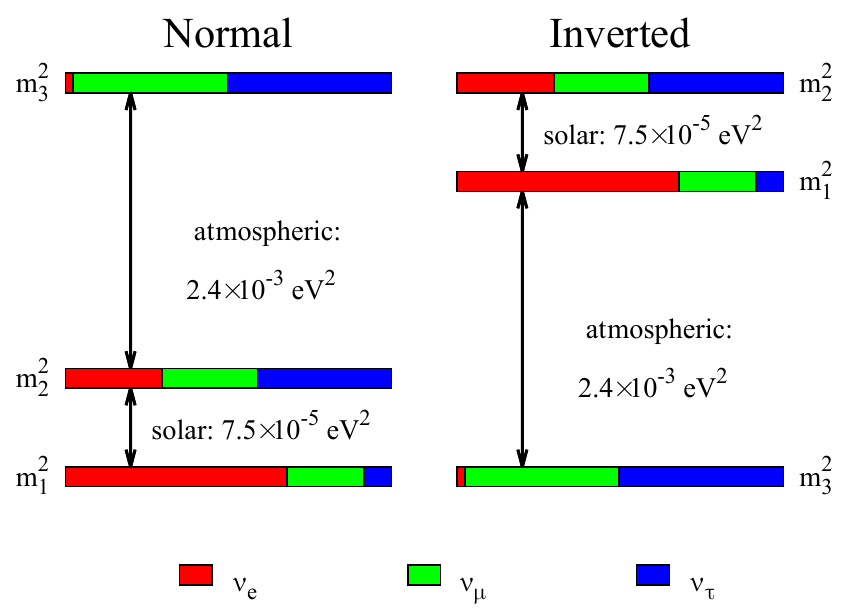
\includegraphics[scale=0.5]{Introduction/massOrdering.png}
  \caption{The two possible \emph{mass hierarchies}, i.e., orderings of neutrino masses, as allowed by current data. From \cite{NuPhysWithJUNO}.}
  \label{fig:massOrdering}
\end{figure}

In an experiment where we are looking for the \emph{disappearance} of (anti)\-neu\-trinos of a given flavor, our interest is in \(P(\alpha \rightarrow \alpha)\). In this case, the behavior of neutrinos and antineutrinos is the same, and \autoref{eq:oscReIm} simplifies to
\begin{equation}
  P(\alpha \rightarrow \alpha) = 1 - 4 \sum_{j>i} |U_{\alpha j}|^2 |U_{\alpha
    i}|^2 \sin^2\left( \frac{\Delta m^2_{ji} L}{4E} \right). 
\end{equation}
The matrix elements from \autoref{eq:upmnsParam} can then be inserted in order to derive the disappearance probability for a particular flavor. For electron antineutrinos, as at Daya Bay, the survival probability is
\begin{align}
  \label{eq:survProbDybFull}
  \begin{split}
    P(\nubar_e \rightarrow \nubar_e) =
    1 &- \cos^4\theta_{13}\sin^2 2\theta_{12} \sin^2 \Delta_{21} \\
    &- \sin^2 2\theta_{13}\left( \cos^2\theta_{12} \sin^2 \Delta_{31} + \sin^2\theta_{12} \sin^2
      \Delta_{32}\right),
  \end{split}
\end{align}
where we've introduced the notation
\begin{align*}
  \Delta_{ji} &\equiv \frac{\Delta m^2_{ji}L}{4E}
           \approx \frac{1.267\, \Delta m^2_{ji}\,\mathrm{[eV^2]}\;
           L\,\mathrm{[m]}}{E\,\mathrm{[MeV]}}.
\end{align*}

Based on the value of $\Delta m^2_{21}$ given in \autoref{tab:pdgOscPars}, at the baselines of Daya Bay \(\sin^2 \Delta_{21}\) is so small that the experiment has no ability to constrain $\theta_{12}$ (nor \(\Delta m^2_{21}\) itself). In this analysis, then, $\theta_{12}$ and $\Delta m^2_{21}$ are fixed to the global values. This leaves $\theta_{13}$, \(\abs{\Delta m^2_{31}}\), and \(\abs{\Delta m^2_{32}}\). However, given that the difference between \(\abs{\Delta m^2_{31}}\) and \(|\Delta m^2_{32}|\) is less than one part in thirty, distinguishing between their corresponding phases would require some combination of a high-resolution detector and a baseline long enough to stretch out the phase difference. At Daya Bay, the baseline of $\sim$1~km is approximately one oscillation length, where the detector resolution is insufficient to resolve the difference. On the other hand, since \(\Delta m^2_{21}\) is well constrained and known to be positive, we can tightly relate \(\abs{\Delta m^2_{31}}\) and \(\abs{\Delta m^2_{32}}\):
\begin{equation}
  \label{eq:hierarchy}
  \abs{\Delta m^2_{31}} =
  \begin{cases*}
    \abs{\Delta m^2_{32}} + \Delta m^2_{21}, & normal hierarchy ($\Delta m^2_{32} > 0$), \\
    \abs{\Delta m^2_{32}} - \Delta m^2_{21}, & inverted hierarchy ($\Delta m^2_{32} < 0$), \\
  \end{cases*}
\end{equation}
Thus, by using this relation to eliminate one parameter, it is possible to perform a two-parameter fit of \autoref{eq:survProbDybFull} directly, \emph{provided that the mass hierarchy is specified}. Since the mass hierarchy is currently unknown, two sets of results must be reported; furthermore, they are subject to change if an improved determination of \(\Delta m^2_{21}\) is ever published.

Alternatively, we can recast \autoref{eq:survProbDybFull} in a form that refers only to an empirical \emph{effective} mass splitting \(\Delta m^2_{ee}\):
\begin{equation}
  \label{eq:survProbDybEE}
  P(\nubar_e \rightarrow \nubar_e) \approx 1 - \cos^4\theta_{13}\sin^2 2\theta_{12} \sin^2 \Delta_{21}
  - \sin^2 2\theta_{13}\sin^2\Delta_{ee},
\end{equation}
where
\begin{equation}
  \Delta_{ee} \equiv \frac{\Delta m^2_{ee}L}{4E}. 
\end{equation}
It must be noted that \autoref{eq:survProbDybEE} is not an exact re-parameterization of \autoref{eq:survProbDybFull}, since the former contains only two frequencies rather than three. Again, however, Daya Bay cannot resolve between $\Delta_{31}$ and $\Delta_{32}$, so there is no practical loss in sensitivity with this approach. The advantage of it is that it produces a single value that is independent of the mass hierarchy and immune to changes wrought by updates to \(\Delta m^2_{21}\).

\(\Delta m^2_{ee}\), as used here, has an \emph{operational,} rather than a physical, definition: It is simply the value that, when inserted into \autoref{eq:survProbDybEE}, gives the best fit to the data.
%
\begin{comment}
  Note that, if Daya Bay only measured antineutrinos at a single $L/E$, we could instead have made a truly physical definition of $\Delta m^2_{ee}$ by declaring that \[ \sin^2 \Delta_{ee} \equiv \cos^2\theta_{12} \sin^2 \Delta_{31} + \sin^2\theta_{12} \sin^2 \Delta_{32}. \] However, the righthand side of this definition depends on $L/E$, so unless this dependence is shown to be negligible, it cannot be used in broadband analyses such as Daya Bay's.
\end{comment}
%
In Daya Bay's case, however, \(\Delta m^2_{ee}\) can be related to physical quantities to a very good degree of approximation. Returning to \autoref{eq:survProbDybFull}, it can be shown \cite{DocDbDm2ee} that, in Daya Bay's range of $L/E$,
\begin{equation}
  \label{eq:dmPhi}
  \cos^2\theta_{12} \sin^2\Delta_{31} + \sin^2\theta_{12}\sin^2\Delta_{32}
  \approx \sin^2 (\Delta_{32} \pm \phi),
\end{equation}
where
\begin{equation}
  \phi \equiv \arctan\left( \frac{\sin2\Delta_{21}}{\cos2\Delta_{21}+ \tan^2
      \theta_{12}} \right),
\end{equation}
and ``+'' (``--'') corresponds to the normal (inverted) hierarchy. Inserting \autoref{eq:dmPhi} into \autoref{eq:survProbDybFull} and comparing to \autoref{eq:survProbDybEE} gives the approximate relation
\begin{equation}
  \label{eq:dmPhiApprox}
  \Delta m^2_{ee} \approx \abs{\Delta m^2_{32}} \pm \Delta m^2_\phi/2,
\end{equation}
where
\begin{equation}
  \Delta m^2_\phi = \frac{4\phi E}{L}.
\end{equation}
Although $\Delta m^2_\phi$ depends on $L/E$, for Daya Bay it is essentially constant and equal to \(\cos^2\theta_{12}\Delta m^2_{21}\). Inserting that into \autoref{eq:dmPhiApprox}, we find that, for both mass hierarchies,
\begin{equation}
  \label{eq:dmPhysical}
  \Delta m^2_{ee} \approx \abs{\Delta m^2_{31}\cos^2\theta_{12}} + \abs{\Delta m^2_{32}\sin^2\theta_{12}}.
\end{equation}
For all intents and purposes, this approximation is exact at Daya Bay. Hence \Autoref{eq:dmPhysical,eq:hierarchy} can be used to relate Daya Bay's measured \(\Delta m^2_{ee}\), as operationally defined by \autoref{eq:survProbDybEE}, to the physical mass splittings for the normal and inverted hierarchies (NH and IH, respectively):
\begin{align}
  \abs{\Delta m^2_{31}} = \Delta m^2_{ee} + \sin^2 \theta_{12} \Delta m^2_{21}, \qquad
  & \abs{\Delta m^2_{32}} = \Delta m^2_{ee} - \cos^2 \theta_{12} \Delta m^2_{21} \qquad
  & \text{[NH]}\\
  % 
  \abs{\Delta m^2_{31}} = \Delta m^2_{ee} - \sin^2 \theta_{12} \Delta m^2_{21}, \qquad
  & \abs{\Delta m^2_{32}} = \Delta m^2_{ee} + \cos^2 \theta_{12} \Delta m^2_{21} \qquad
  & \text{[IH]}
\end{align}
Of course, in doing so, one must still specify the mass hierarchy and \(\Delta m^2_{21}.\) As a sanity check, Daya Bay has compared the results of fitting \autoref{eq:survProbDybFull} and \autoref{eq:survProbDybEE}, finding that, in the end, both techniques give the same values of \(\abs{\Delta m^2_{32}}\) and \(\abs{\Delta m^2_{31}}\). For the sake of simplicity, this analysis will use \autoref{eq:survProbDybEE} and fit \(\Delta m^2_{ee}\).

\section{Further reading}
\label{sec:introFurther}

The history of neutrino oscillations is a fascinating one. For the interested reader, we give a general overview in \autoref{sec:history}. In \autoref{sec:introReactor}, we provide additional historical discussion of reactor neutrino experiments.

\subfilebackmatter

\end{document}
